% !TEX root = ../MasterThesis.tex

\chapter{序論} \label{sec:Introduction}

本章では、最初に1.1節において現在の素粒子物理の基礎となっている、標準理論(Standard Model、 SM)について説明する。その後、1.2節で標準理論を超える理論(Beyond Standard Model, BSM)のいくつかの例を取り上げる。1.3節でBSMを探索する上でカロリメータの果たしうる役割について述べる。1.4節ではその一環として研究が進められている電子陽電子コライダー計画のILC計画について説明する。1.5節ではILC検出器について取り上げる。1.6節ではBSMを電子陽電子ビームによって探索するもう一つの計画であるEBES実験について述べる。1.7節で本研究の目的を説明した後、本論文の流れを概観する。



\section{標準理論}
物質の最も基本的な構成要素とは何か、 という謎は古来から人間の興味を惹きつけるテーマの一つであった。現代ではその基本的な構成要素を素粒子と呼んでいる。20世紀から現在までの素粒子実験により、その性質の多くが標準理論によって記述されることが実証されてきた。

標準理論に属する粒子には大きく分けて4つのグループが存在している。これらを図\ref{StandardModel}
に示す。そのうち、レプトンやクォークは私たちの身の回りの物質を構成する素粒子であり、 スピン1/2のフェルミ粒子である。標準理論には、 6つのレプトンと6つのクォークが存在し、 それぞれ3つの世代に分けられている。世代という言葉は、 レプトンやクォークを分類した時に、 質量の違いによって生じる階層性を示している。それぞれの世代では電荷の違いによって2つの粒子が区別されており、 レプトンでは荷電レプトンと中性レプトン、 クォークでは電荷$+2/3$のクォークと電荷$-1/3$のクォークがそれぞれの世代に含まれている。

標準理論を構成する他の要素がゲージ粒子とHiggsボソンである。ゲージ粒子は現在存在が確かめられている4つの相互作用のうち、 3つを媒介するために必要となる粒子である。4つの相互作用とは、 電磁気相互作用、 弱い相互作用、 強い相互作用、 重力相互作用を指し、これらはゲージ粒子の伝搬が重要な役割を果たす。具体的には、 電磁気相互作用を媒介する光子$\gamma$、強い相互作用を媒介するグルーオン$g$、弱い相互作用を媒介するWボソン($W^\pm$)およびZボソン($Z^0$)が標準理論に含まれる。なお、もう1つのゲージ粒子はグラビトンであり、スピン2を持つとともに重力相互作用を伝搬するが、未だ発見されていない上標準理論の枠組みには当てはまらない。

最後にHiggsボソン$H$の存在は素粒子が質量をもつという事実と関連しており、Higgsボソン自身はスピン0、 電荷0の粒子である。

\begin{figure}[h]
	\begin{center}
		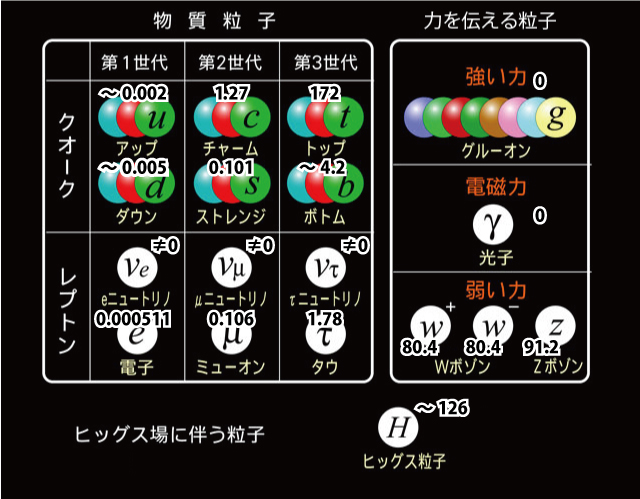
\includegraphics[width=250pt]{./Figure/Introduction/image_01.jpeg}
		\caption[標準模型]{標準模型~\cite{StandardModel}。各粒子の直上に示された数字は質量[GeV]を表す。}
		\label{StandardModel}
	\end{center}
\end{figure}

\section{Beyond the Standard Modelの探索}
標準理論はレプトンやクォークを始めとする素粒子の振る舞いを正確に記述するが、未だこの宇宙には多くの標準理論で説明できない謎が存在している。例として、暗黒物質(Dark Matter, DM)の正体は何か、超高エネルギースケールにおいて力は統一されるのか、ニュートリノの質量の起源とは何か、などが挙げられる。これらの謎に対して、TeVスケールを想定した理論がこれらの謎を解き明かすことが期待されている。一方で、現状のLarge Hadron Collider (LHC)における測定ではこれらの理論で存在が予言される新粒子は発見されていない。そのために、広い視野を持って新たな可能性を探ることが改めて重要となっている。LHCにおける発見が困難な原因として、新物理が重い、新物理で導入される新粒子が強い相互作用をしない、未発見の粒子が縮退した質量スペクトルである、などの要因が存在する可能性がある。もしくは、新粒子が軽いが相互作用の強さが小さいためコライダー実験では検証できない範囲にある可能性も挙げられる。

重心エネルギーが数百$\SI{}{GeV}$を超えるような加速器で粒子衝突を行い、$\SI{}{TeV}$スケール粒子の探索やそれに関連した結合定数などの測定を行う高エネルギー実験と、$\SI{}{GeV}$程度のエネルギーでより高い衝突頻度を持ち、相互作用の小さい$\SI{}{GeV}$スケールの新粒子を探索する固定標的実験は、BSMの広いパラメータスペースを探索する上で相補的に重要である。以下では、そのような新物理の一例を示す。

\subsection{Higgsボソンの精密測定}
2012年にLHCにおいてHiggsボソンが発見され、その存在が証明された。しかし依然としてその詳細な特性は明らかになっていない。例えば、HiggsセクターにおけるHiggsボソンの崩壊分岐比及び質量を極めて精密に測定することは新物理の証拠を見つける上で有力な手法となる。特に、崩壊分岐比を1\%以下の精度まで精密に測定することによりTeVスケールにおける新物理において生じる数\%のSMからのズレを発見することが多くの理論により提唱されている~\cite{Snowmass}。
Higgs質量や崩壊分岐比は表\ref{HiggsDecay}に示す多くの崩壊モードの観測を行うことにより測定される。

\begin{table}[h]
	\begin{center}
		\begin{tabular}{|ccc|}
		\hline
		崩壊モード&分岐比&$\sigma\times BR(\SI{}{fb})$\\\hline\hline
		$h\rightarrow b\bar{b}$&65.7\%&232.8\\\hline
		$h\rightarrow c\bar{c}$&3.6\%&12.7\\\hline
		$h\rightarrow gg$&5.5\%&19.5\\\hline
		$h\rightarrow WW^*$&15.0\%&53.1\\\hline
		$h\rightarrow \tau^+\tau^-$&8.0\%&28.2\\\hline
		$h\rightarrow ZZ^*$&1.7\%&6.1\\\hline
		$h\rightarrow \gamma\gamma$&0.29\%&1.02\\\hline		
		\end{tabular}
	\end{center}
	\caption[Higgsボソンの崩壊モード]{Higgsボソンの崩壊モード}
\label{HiggsDecay}
\end{table}


%%%%%%%%%%%%%%%%%%%%%%%%%%%%%%%%%%%%%%%%%%%%%%%%%%%%%%%%%%%%%%%%%%%%%%%%%%
\begin{comment}
これに加えて、Higgs-strahlung (図\ref{Higgs})により生成されるHiggsボソンの情報は崩壊分岐比を測定する上で重要な要素の一つである。この反応では、HiggsボソンはZボソンの反跳粒子として得られるので、Higgsボソンの崩壊モードによらずZボソンの崩壊にのみ着目することでヒッグス粒子の任意の粒子への崩壊断面積$\sigma_{ZH}\times BR\ (H\rightarrow X)\ (X = b, W, \tau, \ldots)$の測定を行うことができる。
\end{comment}
%%%%%%%%%%%%%%%%%%%%%%%%%%%%%%%%%%%%%%%%%%%%%%%%%%%%%%%%%%%%%%%%%%%%%%%%%%


\begin{figure}[h]
	\begin{center}
		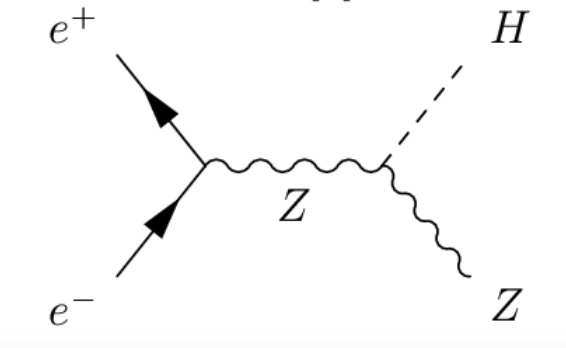
\includegraphics[width=150pt]{./Figure/Introduction/eeZZH.png}
		\caption[Higgs-strahlungのファインマンダイアグラム]{Higgs-strahlungのファインマンダイアグラム}
		\label{Higgs}
	\end{center}
\end{figure}

\subsection{超対称性}
超対称性は新物理探索の中で最も有望視され、これまでのコライダー実験でその理論に基づく新粒子の探索が行われてきた。SM粒子のパートナーとして、スピンが$1/2$だけ異なる超対称性パートナーを仮定し、RパリティやSMパートナーとの結合定数などのパラメータを考慮する。Rパリティは
\[
R\equiv(-1)^{3(B-L)+2S}
\]
によって定義される値で、超対称性粒子は$R=-1$、SM粒子は$R=1$をもつ。ここで、$S$はスピン、$B$はバリオン数、$L$はレプトン数である。

超対称性粒子の主な例を表\ref{SUSY_particle}に示す。%これらの他に、荷電Winoと荷電Higgsinoの混合状態である Chargino ($\chi^\pm$)やZino、Photinoと中性Higgsinoの混合状態であるNeutralinoが挙げられる。

\begin{table}[H]
	\begin{center}
		\begin{tabular}{|ccc|}
		\hline
		フェルミオン&超対称性パートナー&超対称性パートナーを示す記号\\\hline\hline
	        electron&selectron&$\tilde{e}$\\\hline
	        muon&smuon&$\tilde{\mu}$\\\hline
	        tauon&stauon&$\tilde{\tau}$\\\hline
	        electron neutrino&electron sneutrino&$\tilde{\nu_e}$\\\hline
	        muon neutrino&muon sneutrino&$\tilde{\nu_\mu}$\\\hline
	        tau neutrino&tau sneutrino&$\tilde{\nu_\tau}$\\\hline
	        up quark&scalar up quark&$\tilde{u}$\\\hline
	        down quark&scalar down quark&$\tilde{d}$\\\hline
	        charm quark&scalar charm quark&$\tilde{c}$\\\hline
	        strange quark&scalar strange quark&$\tilde{s}$\\\hline
	        top quark&scalar top quark&$\tilde{t}$\\\hline
	        bottom quark&scalar bottom quark&$\tilde{b}$\\\hline
	        \hline
	        ゲージボソン&超対称性パートナー&超対称性パートナーを示す記号\\\hline\hline
	        photon&photino&$\tilde{\gamma}^0$\\\hline
	        gluon&gluino&$\tilde{g}$\\\hline
	        W Boson&wino&$\tilde{W}^\pm$\\\hline
	        Z Boson&zino&$\tilde{Z}^0$\\\hline
	        %Higgs Boson&higgsino&$\tilde{H}^0,\tilde{H}^\pm$\\\hline
	        \hline
		\end{tabular}
	\end{center}
	\caption[超対称性パートナーの例]{超対称性パートナーの例。}
\label{SUSY_particle}
\end{table}

%%%%%%%%%%%%%%%%%%%%%%%%%%%%%%%%%%%%%%%%%%%%%%%%%%%%%%%%%%%%%%%%%%%%%%%%%%%%%%%%%%%
\begin{comment}
\begin{table}[H]
	\begin{center}
		\begin{tabular}{|ccc|}
		\hline
		フェルミオン&超対称性パートナー&超対称性パートナーを示す記号\\\hline\hline
	        電子(electron)&スカラー電子(selectron)&$\tilde{e}$\\\hline
	        ミューオン(muon)&スカラーミューオン(smuon)&$\tilde{\mu}$\\\hline
	        タウオン(tauon)&スカラータウオン(stauon)&$\tilde{\tau}$\\\hline
	        電子ニュートリノ(electron neutrino)&スカラー電子ニュートリノ(electron sneutrino)&$\tilde{\nu_e}$\\\hline
	        ミューニュートリノ(muon neutrino)&スカラーミューニュートリノ(muon sneutrino)&$\tilde{\nu_\mu}$\\\hline
	        タウニュートリノ(tau neutrino)&スカラータウニュートリノ(tau sneutrino)&$\tilde{\nu_\tau}$\\\hline
	        アップクォーク(up quark)&スアップスクォーク(scalar up quark)&$\tilde{u}$\\\hline
	        ダウンクォーク(down quark)&スダウンスクォーク(scalar down quark)&$\tilde{d}$\\\hline
	        チャームクォーク(charm quark)&スチャームスクォーク(scalar charm quark)&$\tilde{c}$\\\hline
	        ストレンジクォーク(strange quark)&スストレンジスクォーク(scalar strange quark)&$\tilde{s}$\\\hline
	        トップクォーク(top quark)&ストップスクォーク(stop squark)&$\tilde{t}$\\\hline
	        ボトムクォーク(bottom quark)&ボトムクォーク(s squark)&$\tilde{d}$\\\hline
	        \hline
	        ゲージボソン&超対称性パートナー&超対称性パートナーを示す記号\\\hline\hline
	        光子(photon)&ヴィーノ(Bino)&$\tilde{B_0}$\\\hline
	        グルーオン(gluon)&グルイーノ(gluino)&$\tilde{g}$\\\hline
	        Wボソン(W Boson)&ウィーノ(wino)&$\tilde{W}^\pm$\\\hline
	        Z ボソン(Z Boson)&グルイーノ(zino)&$\tilde{W}^0$\\\hline
	        Higgs ボソン(Higgs Boson)&ヒッグシーノ(higgsino) &$\tilde{H}$\\\hline
	        \hline
		\end{tabular}
	\end{center}
	\caption[超対称性パートナーの例]{超対称性パートナーの例。}
\label{SUSY_particle}
\end{table}

\end{comment}
%%%%%%%%%%%%%%%%%%%%%%%%%%%%%%%%%%%%%%%%%%%%%%%%%%%%%%%%%%%%%%%%%%%%%%%%%%%%%%%%%%%%%%

さらに、GauginoおよびHiggsinoが混合して生じるcharginoやneutralinoの存在も予測されている。

超対称性粒子はその質量の順序に関して幾つかの仮説があるが、最も軽い超対称性粒子(the Lightest SUSY Particle、 LSP)としては通常Nuetralinoが考えられる。Neutralinoの混合として、Wino-likeもしくはHiggsino-likeとして存在している場合、LSPと質量差がほとんど無いBosinoが存在することが示唆されている。一方、Bino-likeなNeutralinoがLSPである場合、LSPと次に軽い超対称性粒子との間に大きな質量差が生じる。しかし、この場合、初期宇宙のLSP生成および消滅の間にバランスが必要になるため、DMの存在が予期される。SUSY粒子の消滅を高めるための方法として$\tilde{\tau}$の対消滅を通じて生成するものがある。

SUSYは$\ \SI{}{GeV} - \ \SI{}{TeV}$まで探索が行われているが、未だ発見されておらず質量や結合定数に対する制限が与えられている。そのため、現在さらに高エネルギー領域へと探索範囲が広げられつつある。

加速器でSUSYを探索する上で、コライダー実験で SUSY を探索する上で、R パリティが保存するモデルを考えると、最終状態に必ず偶数個のLSPが現れる。
SUSY粒子のカスケード崩壊\footnote{粒子が物質中に入射すると連続的に相互作用を引き起こす。これをカスケード崩壊と呼ぶ。第2章で詳しく述べる。}で現れるSM粒子の信号と、LSPによるエネルギー・運動量欠損からSUSY探索を行う。

\subsection{Axion/ALPs}
BSMでその存在が予想されている粒子の一つに擬スカラー粒子が挙げられる。この粒子は物理学における強いCP問題の解を探索する上で提案された~\cite{Axion}~\cite{Axion1}。  quantum chromodynamics (QCD)におけるLagrangianは
%\begin{equation}
\[
{\cal L}_{QCD} = \sum_{q} \bar{q}(i \cancel D - m_q e^{i\theta_q \gamma_5})q -\frac{1}{4} G^{a \mu\nu}G^a_{\mu\nu} + \theta \frac{g_s^2}{32\pi^2}G^{a\mu\nu}\tilde{G}^a_{\mu\nu}
%\end{equation}
\]
と記される。ここで、$\theta_q$および$\theta$はそれぞれクォーク質量の位相およびゲージ変換における定数である。これらの定数はPおよびT変換に対して保存しないので、一般にはQCDにおけるCP対称性の破れが生じると考えられていた。しかし、中性子の電気双極子モーメント$d_n$の測定から得られる$\theta_q + \theta$の値はこの予測値よりも小さく、従ってCP破れの程度が小さくなることが示されている。これを強いCP問題と呼ぶ。

この問題の解の一つとして与えられたのが擬スカラー粒子のQCD axionである。もしこの粒子が存在すると仮定すれば、QCDラグランジアンは
\begin{equation}
{\cal L} = \left(\frac{a}{f_a} - \bar{\theta}\right) \frac{\alpha_s}{8\pi }G^{\mu\nu a}\tilde{G}^a_{\mu\nu} 
\end{equation}

\[
a : \textrm{QCD axion}
\]
\[
\bar{\theta} = \theta_q + \theta
\]
となり、$\bar{\theta}$の項が相殺されるため、CP保存が成立する。Axionの質量の候補としては$\SI{}{\mu eV}$ 程度の極めて小さいものから TeV スケール以上の大きいものまで幅広く、もし十分に小さいのであれば、高エネルギー加速器を使用することなく、小規模の実験でも発見されうる。Axionを探索するための実験は今日まで行われてきているが、未だ発見されていない。

Axionと同様に自発的対称性の破れから生じる擬南部ゴールドストーン粒子をAxion Like Particles (ALPs)と呼び、これらの粒子もまた探索の対象となっている。ALPsは多くの理論により予言されており、その質量や結合の強さは様々に及んでいる。一つのモデルとして、次の有効ラグランジアンによって記述されるALPが提案されている。
\begin{equation}
\delta{\cal L} =-\frac{1}{4}g_{a\gamma\gamma}aF_{\mu\nu}\tilde{F}^{\mu\nu}+\frac{1}{2}(\partial_{\mu}a)^2-\frac{1}{2}m_a^2a^2
\end{equation}

ここで$a$はALPを指しており、$F$はフォトン場の強さ、$\tilde{F}^{\mu\nu}=\epsilon_{\mu\nu}\lambda_\rho F^{\lambda\rho}/2$である。
このALPの角度に対する生成微分断面積は
\begin{equation}
\frac{d\sigma_{\gamma a}}{d\theta_a} \cong \frac{\alpha g^2_{a\gamma\gamma}k^4\theta_a^3}{t4^2} G_2(t)
\end{equation}
で表される。ここで、$G_2(t)\cong Z^2(a'^2t/(1+a7^2t))^2/(1+t/d)^2$、$Z$は標的の原子番号、$a'=112Z^{-1/3}/m_e$、$d=\SI{0.164}{GeV^2}$、$m_e=\SI{511}{keV}$は電子質量である。
一方、崩壊幅は
\begin{equation}
\Gamma_a = \frac{g_{a\gamma\gamma^2 m_a^3}}{64\pi}
\end{equation}
であり、2光子へと崩壊する。電子ビームのビームダンプへの照射からALPが生成されるファインマンダイアグラムを図\ref{ALP_int}に示す。aがALPを示しており、その崩壊で生じる2光子対をカロリメータによって検出する。

\begin{figure}[h]
	\begin{center}
		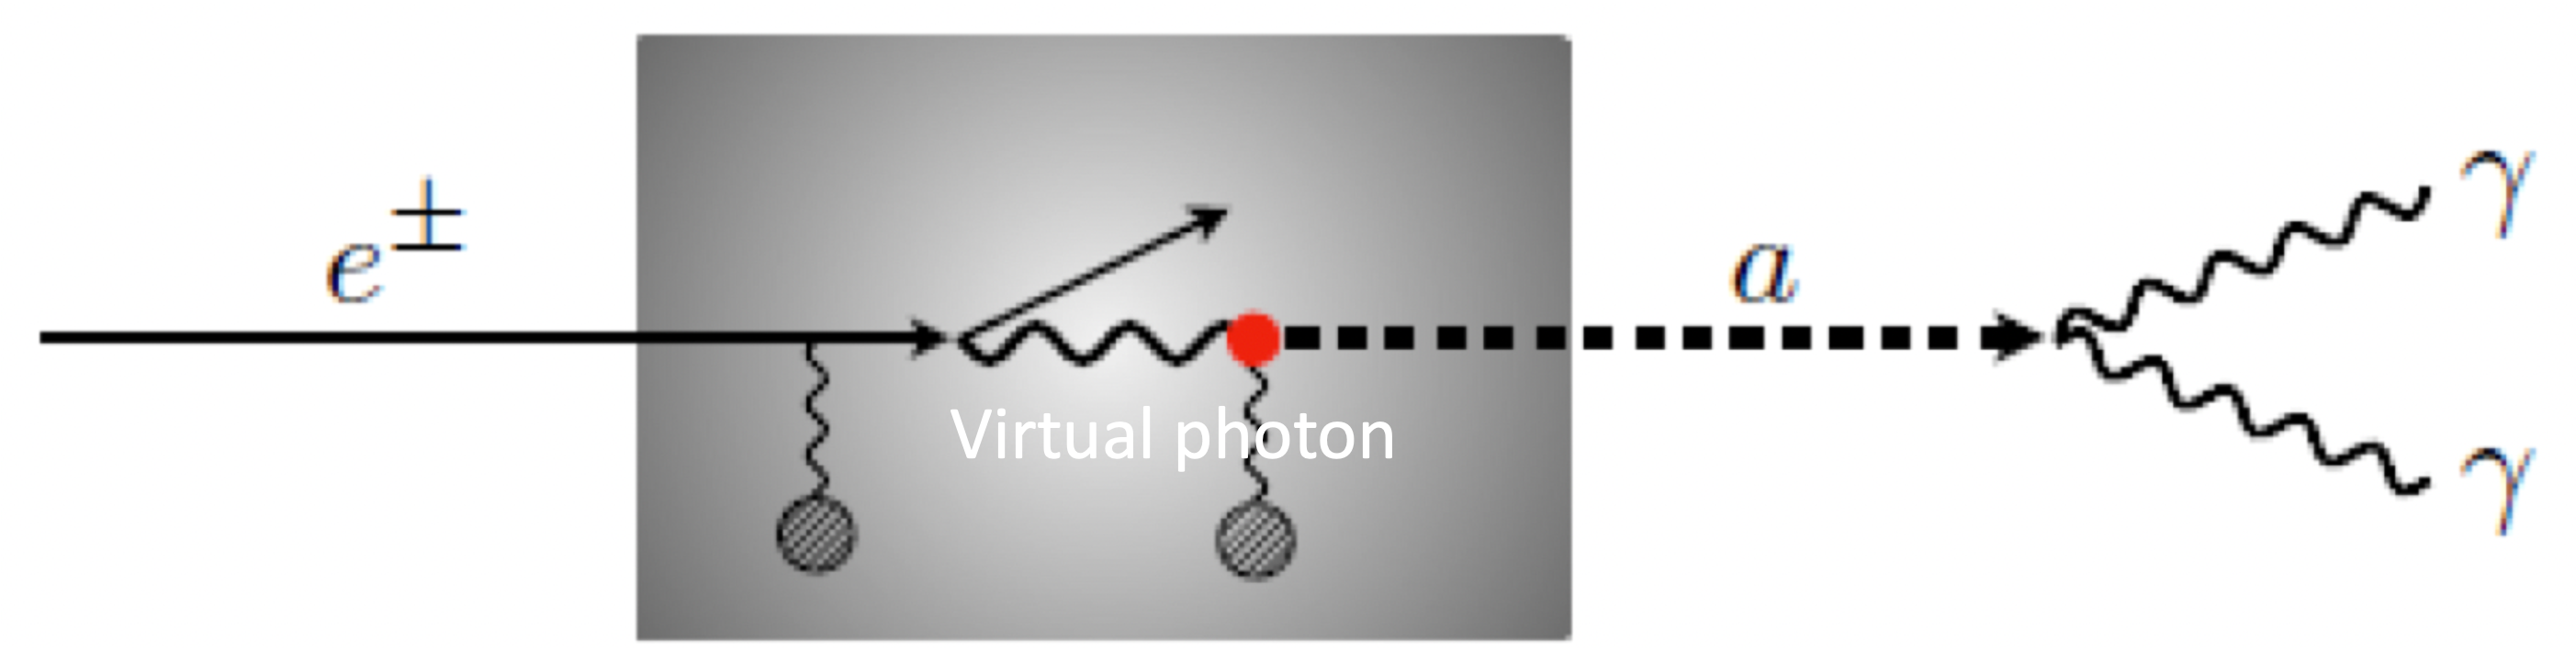
\includegraphics[width=350pt]{./Figure/Introduction/ALP_int.png}
		\caption[ビームダンプによるALPの生成を示すファインマンダイアグラム]{電子ビームのビームダンプによるALPの生成を示すダイアグラム。aがALPを示している。}
		\label{ALP_int}
	\end{center}
\end{figure}


%この粒子は強いCP問題のPeccei-Quinn解の候補として得られ、QCD Axionと名付けられた。Axionは初期宇宙において冷たいDMとして残存しうることが宇宙論の観測から推測され、現在のダークマター候補の一つとして有力視されている。

%これらの事実から、LHCで見つかりにくい新物理に感度がある$e^+e^-$ Higgs Factoryと結合が小さい新物理を探せる固定標的実験の両面で新物理を探索する必要がある。

%今回の研究では$e^+e^-$ Higgs factoryと$e^+e^-$固定標的実験の双方で、共通の技術を使うことができるカロリメーター技術に着目し、その実装と各実験での応用を検討した。
%例えば、ダークマターが挙げられる。この物質はエネルギー密度に関して宇宙の構成要素の25\%を占めると推定され、このダークセクターに属する粒子は標準理論のSM粒子と非常に弱く相互作用するため、検出が難しいと考えられている\cite{Axion}。現在までに数々のSMを超える理論(Beyond Standard Model、 BSM)が発表され、この粒子の特性を予想している。

\section{新物理探索におけるカロリメータの役割}
新物理イベントが生じていれば、特定のイベントに対して実験で測定される散乱断面積に標準理論で記述される散乱断面積とのズレが生じ、そのズレを精度よく測定することによって新物理が存在することがより強く示唆される。新物理探索を行う上でのカロリメータの役割はビームの衝突によって生じたジェットや中性粒子を特定し、そのエネルギーを測定することである。
%%%%%%%%%%%%%%%%%%%%%%%%%%%%%%%%%%%%%%%%%%%%%%%%%%%%%%%%%%%%%%%%
\begin{comment}
カロリメータで測定されたジェットエネルギーは解析を通じて再構成され、不変質量へと変換される。不変質量$m_0$は光速$c$、粒子のエネルギーを$E$、粒子の運動量を$\mathbf{p}$とすると、以下の式で表される。
\begin{equation}
(m_0c^2)^2 =E^2-c^2|\mathbf{p}|^2
\end{equation}

%モンテカルロ(MC)シミュレーションはハードウェアでは観測できないバックグラウンド事象を推定するために有効であり、新物理探索を行う上では必要不可欠である。
%シミュレーションを元にした不変質量分布により、バックグラウンド事象とシグナル事象が区別され、もしここで新物理が観測できていれば、SMに基づいたシミュレーションでは存在しないスペクトラムが現れている。
\end{comment}
%%%%%%%%%%%%%%%%%%%%%%%%%%%%%%%%%%%%%%%%%%%%%%%%%%%%%%%%%%%%%%%
新物理探索を行う上で必要となるのがジェットエネルギー分解能の向上である。
%再構成される不変質量スペクトラムには事象由来の自然幅に加えて、統計量の平方根に依存する統計誤差と測定器に依存する系統誤差が生じる。この影響により断面積の小さい反応はもし観測できていたとしてもピークが埋没してしまい存在を確認することが難しくなる。
例として、ILC計画においてW - Zボソンの不変質量を3$\sigma$の精度で識別するためには角度の不確定性を無視すると少なくとも3-4\%のジェットエネルギー分解能を必要とする~\cite{PFATest}。
この精度はハードウェアの改善だけでなく、ソフトウェアによる解析アルゴリズムの改善が必要不可欠である。

%新物理が観測された証明をより確固たるものとするためにはルミノシティを高め、統計誤差を減らすだけでなく、検出器や検出アルゴリズムに依存した系統誤差を低減させることが重要となる。
%その上で課題となるのが、粒子の識別精度やバックグラウンドとの分離などである。相互作用によって生じた粒子が崩壊して検出器に入射した時、そのタネとなる粒子の種類が異なっていても、検出器により取得された情報だけでは同定が困難なケースが存在する。

\begin{comment}
\begin{itemize}
\item PFAを用いてジェットエネルギー分解能の向上させることによりTPCにおいて荷電粒子のエネルギーをより精度良く測定する
\item Ecalにおいて入射する光子のエネルギーをより精度良く測定する
\end{itemize}
の2つが挙げられる。
\end{comment}

\section{ILC計画}
国際リニアコライダー計画(International Linear Collider、 ILC)はHiggsボソンの詳細な特性を解明し、新物理探求を行うことを主目的とした次世代の電子陽電子直線加速器計画である。その概形は図\ref{ILCaccelerator}に示されている。建設予定地は東北地方の北上山地であり、安定した地盤とトンネル掘削のしやすさを特徴としている。ILCはその名の通り世界中の研究者が共同で実験計画および実行を行う国際プロジェクトとして進行しており、世界各地の研究機関で加速器や各検出器などの開発が行われている。

\begin{figure}[h]
	\begin{center}
		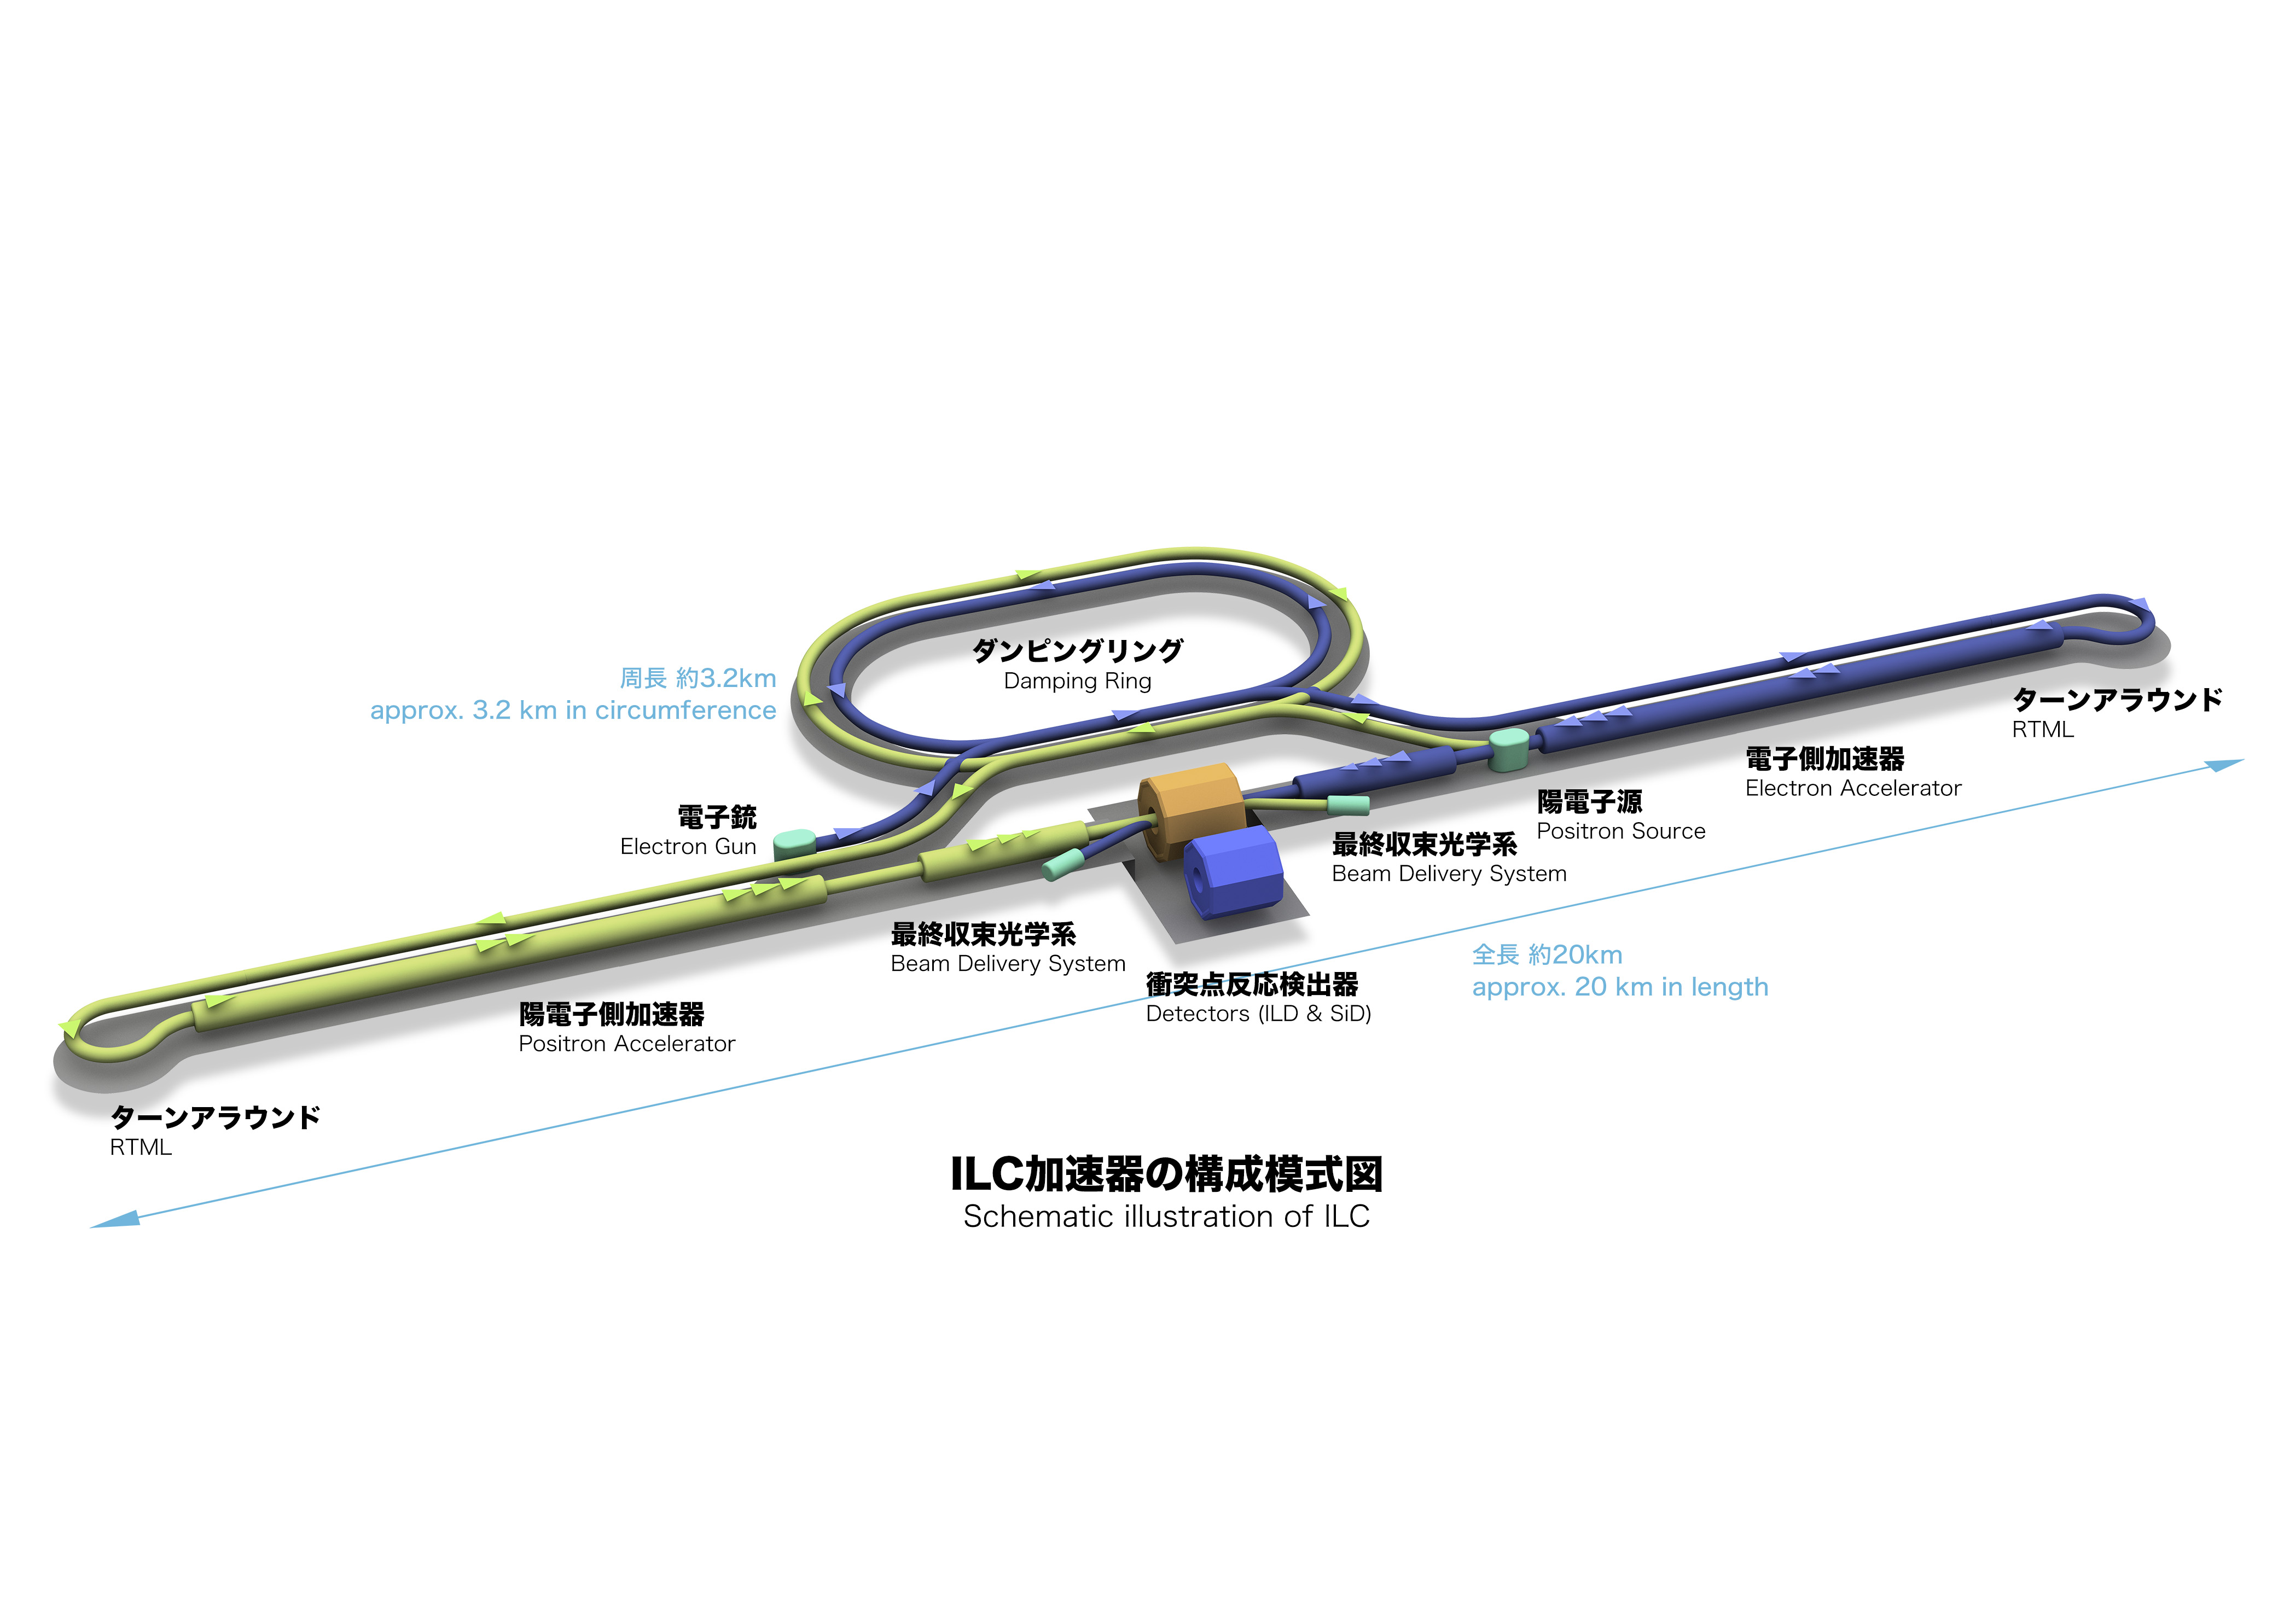
\includegraphics[width=350pt]{./Figure/Introduction/image_02.jpg}
		\caption[ILC加速器]{ILC加速器~\cite{StandardModel}。}
		\label{ILCaccelerator}
	\end{center}
\end{figure}


ILCは電子陽電子直線加速器を有するという特徴から、同じ高エネルギー実験である陽子陽子円形加速器Large Hadron Collider (LHC)にない長所を持ち、異なる役割を果たす。

ILCの運転開始時はHiggsボソン生成を起こすために最適のエネルギーである$\SI{250}{GeV}$の重心系エネルギーで陽電子と電子を衝突させる。これはHiggsボソンの質量がおよそ$\SI{125}{GeV}$であることに由来する。直線型加速器は円形加速器と異なり、加速器直線部分の延長、もしくは加速技術の向上によって$\SI{1}{TeV}$以上のエネルギーまで拡張可能である。

さらに、円形加速器では重心系エネルギーの増加に伴って制動放射によるエネルギーロスの増大が発生し大きな課題となるが、線形加速器ではその影響が無く、十分に高いエネルギーまでエネルギーロスを少なく加速を行うことを可能とする。

また、LHCでは陽子が強い相互作用に伴う反応を引き起こすために非常に多くのバックグラウンドの影響を受けるが、ILCは素粒子である陽電子と電子のコライダーであるためにその影響が相対的に少なくて済むため、精密測定や稀な崩壊を観測することに長所を持つ。

一方で、円形コライダーは繰り返し周回して粒子衝突を行うことが可能であるが、ILCは直線加速器のため粒子の衝突は1回のみである。そのため、ルミノシティを上げてイベントの生成回数を高める必要があり、電子および陽電子のビームは十分にエミッタンスを絞って衝突が引き起こされる。ルミノシティとは、ビーム衝突型加速器におけるビーム衝突回数を示した値で、単位時間当たりの反応数を$N$、断面積を$\sigma$とすると、単位時間当たりのルミノシティ$L$は、
\begin{equation}
L = \frac{N}{\sigma}
\end{equation}
で表される。

ILCの加速器には高純度ニオブを用いた超伝導加速空洞が使用される。超伝導は極低温において電流の流れる際の抵抗値が極めて0に近くなる現象である。これにより、加速空洞中の表面において消費されるエネルギーを低減させることができる。この影響を低減することは、超伝導を実現するための冷却に必要となる電力を差し引いても大きなメリットである。加速空洞は図\ref{cavity}に示すように9つのセルが接合された構造を持ち、内部で電場を構成することにより粒子ビームを加速させる。さらに、超伝導現象を引き起こすために液体ヘリウムによって極低温に保たれている。

\begin{figure}[h]
	\begin{center}
		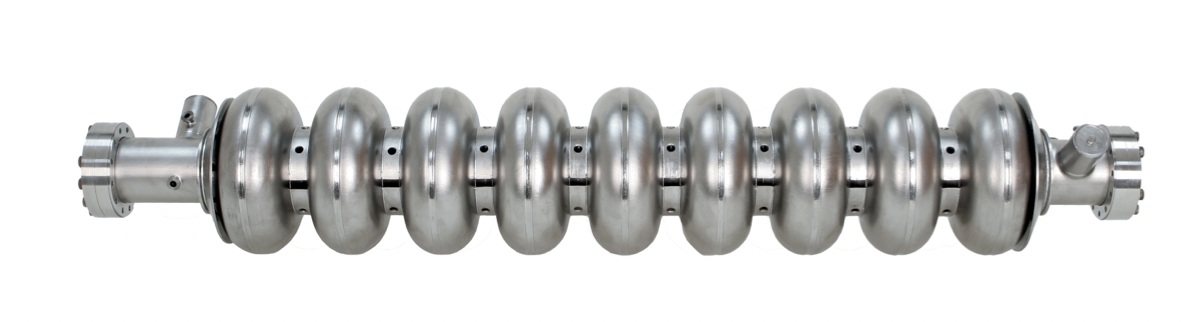
\includegraphics[width=250pt]{./Figure/Introduction/cavity.png}
		\caption[ILC超伝導加速空洞]{ILC超伝導加速空洞}
		\label{cavity}
	\end{center}
\end{figure}


\begin{comment}
\section{ILCの物理}
ILCの運転開始エネルギーである$\SI{250}{GeV}$では、先ほど述べたようにHiggsボソン生成過程であるZh随伴過程が主要な寄与を示す。この散乱断面積を図\ref{ZhCrossSection}に示す。エネルギーの増加とともに徐々にWW fusionの断面積も増大し、エネルギーアップデート後の実験ではこの寄与も重要となる。Zh随伴生成の有益な点としては、ZボソンがHiggsボソンの反跳として生じるため、Higgsボソンの直接観測をすることなくその分岐比や質量を測定することが可能な点である。

\begin{figure}[h]
	\begin{center}
		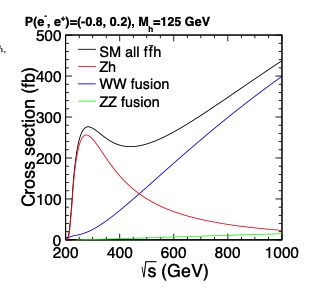
\includegraphics[width=250pt]{./Figure/Introduction/image_03.jpg}
		\caption[重心系エネルギー$\SI{250}{GeV}$付近の主要過程の断面積]{重心系エネルギー$\SI{250}{GeV}$付近の主要過程の断面積}
		\label{ZhCrossSection}
	\end{center}
\end{figure}

Zh随伴過程などのプロセスにより生成されたHiggsボソンはさまざまな崩壊モードを持ち、その一覧が表\ref{HiggsDecay}に示されている~\cite{ILCPhysics}。

\begin{table}[h]
	\begin{center}
		\begin{tabular}{|c|c|c|}
		\hline
		崩壊モード&分岐比&$\sigma\cdot BR(\SI{}{fb})$\\\hline\hline
		$h\rightarrow b\bar{b}$&65.7\%&232.8\\\hline
		$h\rightarrow c\bar{c}$&3.6\%&12.7\\\hline
		$h\rightarrow gg$&5.5\%&19.5\\\hline
		$h\rightarrow WW^*$&15.0\%&53.1\\\hline
		$h\rightarrow \tau^+\tau^-$&8.0\%&28.2\\\hline
		$h\rightarrow ZZ^*$&1.7\%&6.1\\\hline
		$h\rightarrow \gamma\gamma$&0.29\%&1.02\\\hline		
		\end{tabular}
	\end{center}
	\caption[Higgsボソンの崩壊モード]{Higgsボソンの崩壊モード。}
\label{HiggsDecay}
\end{table}

Higgsボソンに関する重要な測定として、質量および生成断面積、崩壊分岐比がある。これらのパラメータを精密に測定することは、LHCで観測された$\SI{125}{GeV}$の共鳴が標準理論にあるHiggsボソンと一致するのか、それとも別の構造を持った粒子なのかという重要な問いに答えるために必要となる。

\begin{figure}[h]
	\begin{center}
		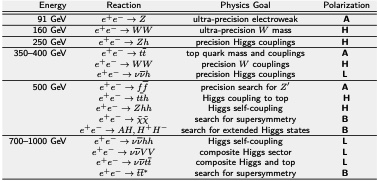
\includegraphics[width=370pt]{./Figure/Introduction/image_04.jpg}
		\caption[各重心系エネルギーで主要となる過程]{各重心系エネルギーで主要となる過程}
		\label{DominantProcess}
	\end{center}
\end{figure}

\begin{table}[h]
	\begin{center}
		\begin{tabular}{cccc}
		\hline
		エネルギー&過程&物理目標\\\hline
		$\SI{91}{GeV}$&$e^+e^-\rightarrow Z$&電弱精密測定\\
		$\SI{160}{GeV}$&$e^+e^-\rightarrow WW$&W質量精密測定\\
		$\SI{250}{GeV}$&$e^+e^-\rightarrow Zh$&Higgs結合精密測定\\
		$350 - \SI{450}{GeV}$& $e^+e^-\rightarrow t \bar{t}$&tクォークの質量および結合定数精密測定\\
		\end{tabular}
	\end{center}
	\caption[各重心系エネルギーで主要となる過程の表]{各重心系エネルギーで主要となる過程の表}
\label{DominantProcess_table}
\end{table}
\end{comment}


\section{ILC検出器}
ILC加速器の衝突点にはILD (International Large Detector)とSiD (Silicon Detector)の2種類の検出器が置かれることが計画されている。それぞれの検出器に含まれる構成はほぼ同じだが、一つの違いとしてILDは飛跡検出器にTPCとシリコン検出器を用いている一方で、SiDは飛跡検出器全体がシリコン検出器であることが挙げられる。ILDとSiDのそれぞれの検出器が独立に測定を行い、実験の信頼性の向上を図っている。本研究はこのうち、ILDを対象としている。
加速器実験に使用される大型の検出器は、一つの装置で非常に多くの種類データを測定するためにさまざまなモジュールを搭載した複合検出器として設計される。ILDに含まれる主な構成要素が表\ref{Detector}に挙げられている。

飛跡検出はVTX、SITおよびTPCで測定されたデータを基に解析が行われる。ILC計画においてはbクォークとcクォークの測定が非常に重要となり、高精度のフレーバーの特定が要求される。この解析をflavor taggingと呼ぶ。これらのクォークは相対論的効果を無視するとかなり短い距離($b$クォークは$400-\SI{500}{\mu m}$、$c$クォークは$20-\SI{300}{\mu m}$)しか走らないという特性から、飛跡検出器はビーム相互作用点からおよそ$\SI{1.6}{cm}$の非常に近い位置に置かれ、$\SI{3}{\mu m}$以下の高精度の位置分解能を持つように設計されている。

ECALおよびHCALからなるカロリメータでは光子および電子、中性ハドロンのエネルギー測定を行う。カロリメータについては第2章で詳しく述べるが、大きな特徴としてそれぞれのレイヤーを非常に微細化しており、高い位置分解能での測定を可能としている。

検出器だけでは入射してくる荷電粒子の運動量を求めることはできないため、ソレノイドを用いて入射粒子の軌道を曲げることが必要となる。ILDでは$\SI{3.5}{T}$超伝導ソレノイドを利用する。このソレノイドによって生じた磁場は入射粒子の運動量に応じて曲率半径が変化し、この半径を測定することで運動量を求めることが可能となる。また、Iron Yokeはミューオンとそれ以外の粒子を識別するために磁場によって生じたflux returnの影響からソレノイドの磁束が拡散するのを防ぐことを主目的とする。
%また、電源装置などによって生じる外部磁場が問題となるため、Iron Yokeを配置してそれらの影響を低減させる。
%その他にも、入射した粒子の運動量を知るために磁場によって曲げられた曲率を測定するための$\SI{3.5}{T}$超伝導ソレノイドや、外部から侵入してくる磁場の影響を低減させるためのIron Yokeが備えられる。

%ビームモニターには、表\ref{BeamMonitor}に示される検出器群が用いられる。ビームには高いルミノシティが要求されるため、加速器稼働中はその状態が一定となっていることを確認することが重要である。


\begin{table}[h]
	\begin{center}
		\begin{tabular}{c|c|c}
		\hline
		検出器名&検出器略称&役割\\\hline\hline
		Vertex Detector&VTX&崩壊点検出\\
		Silicon Internal Tracker&SIT&崩壊点付近の飛跡検出\\
		Time Projection Chamber&TPC&飛跡検出\\
		Electromagnetic Calorimeter& ECAL&電子および光子のジェットエネルギー測定\\
		Hadron Calorimeter&HCAL&中性ハドロンのジェットエネルギー測定\\\hline
		\end{tabular}
	\end{center}
	\caption[ILDに導入される検出器モジュール]{ILCに導入される検出器モジュール}
\label{Detector}
\end{table}

\begin{comment}
\begin{table}[h]
	\begin{center}
		\begin{tabular}{cccc}
		\hline
		検出器名&検出器略称&役割\\\hline
		VTX&Vertex Detector&崩壊点検出\\
		Silicon Internal Tracker&SIT&崩壊点付近の飛跡検出\\
		Time Projection Chamber&TPC&飛跡検出\\
		Electromagnetic Calorimeter& ECAL&電子および光子のジェットエネルギー測定\\
		\end{tabular}
	\end{center}
	\caption[ILC加速器に備えられるビームモニター]{ILC加速器に備えられるビームモニター}
\label{BeamMonitor}
\end{table}
\end{comment}



\section{EBES実験}
Electron Beam dump Experiment at Switchyard 3 (EBES)実験は茨城県・高エネルギー加速器研究所にあるSuper KEKB Linacを用いてALPsを探索することを目的とした実験である。実験はSuper KEK  LinacのSwitching yard 3 (SY3)で行われる。この実験では、電子・陽電子ビームをビームダンプへと入射させ、内部で仮想光子が生じた後、ALPsへと崩壊するイベントを観測する。ALPsはビームダンプを通過して光子ペアへと崩壊するため、直接観測が可能となる。Linac は$\SI{4}{GeV}$までの陽電子ビームと$\SI{7}{GeV}$までの電子ビームが利用可能である。

実験により排除される領域に関して、他の実験と比較したのが図\ref{ALP_world}である~\cite{EBES}。

\begin{figure}[h]
	\begin{center}
		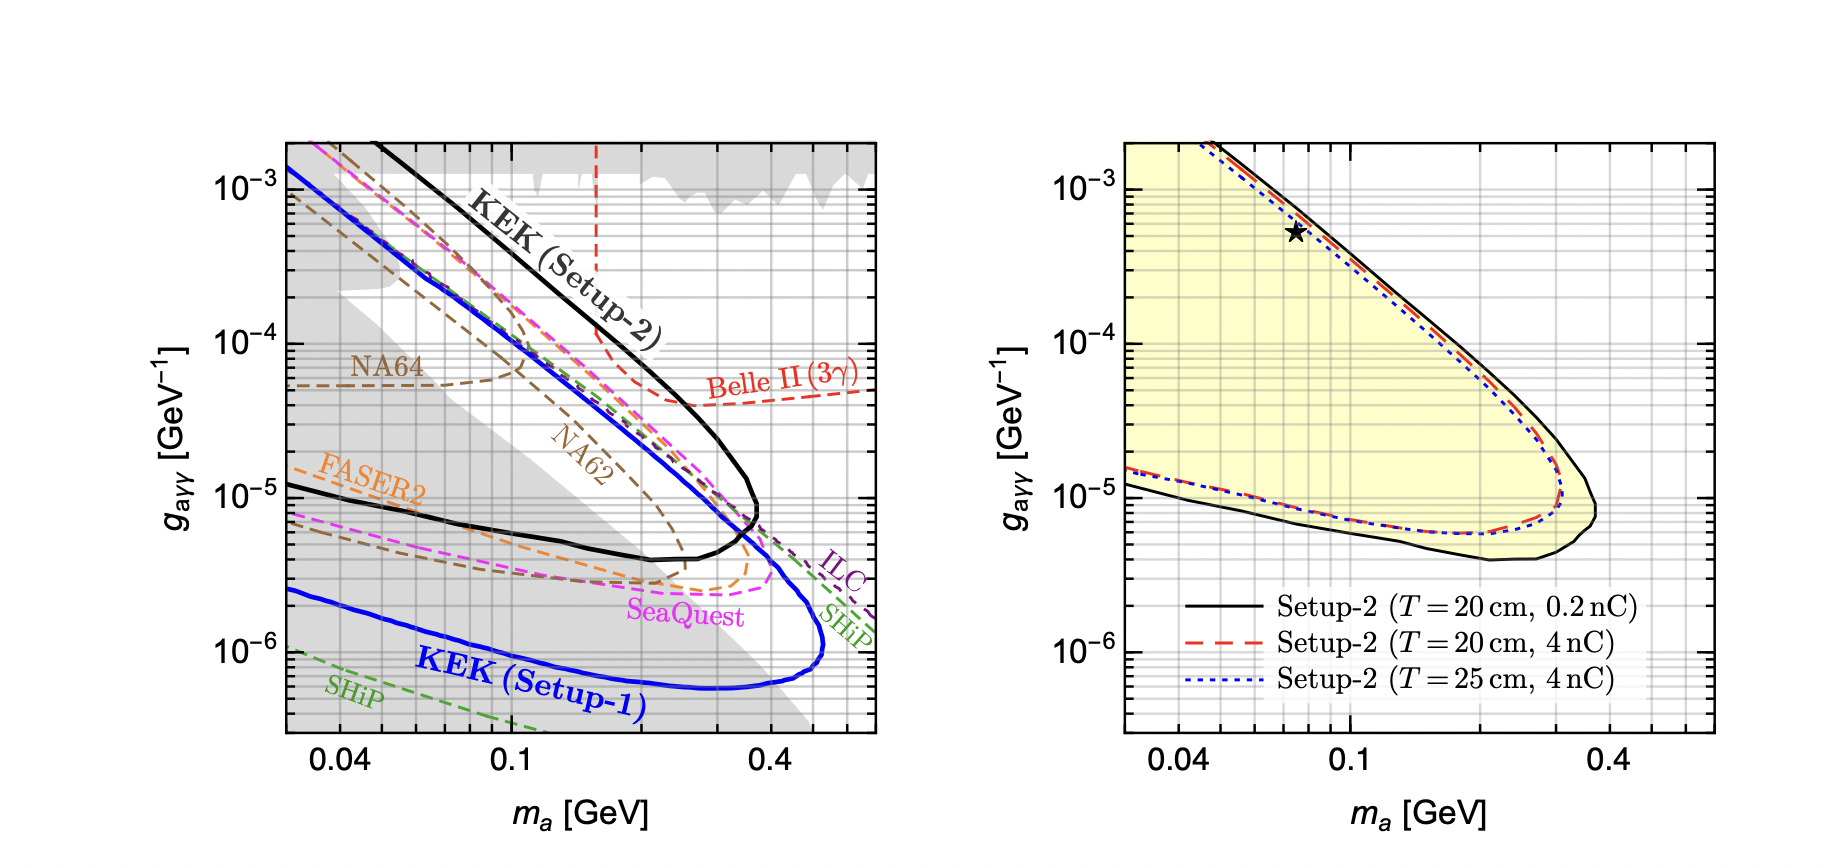
\includegraphics[width=370pt]{./Figure/Introduction/ALP_world.png}
		\caption[EBES実験によるALPの95\%C.L.]{EBES実験によるALPの95\%C.L.。ALPsの結合定数および質量について示されている。左図は他の実験との比較で、右図は第5章で説明するSetup-2の変更による差を表している。}
		\label{ALP_world}
	\end{center}
\end{figure}

SHiPやFASER2などの実験と比較すると、より短寿命のALPsをより低コストで探索することが本実験の特徴の一つである。

\section{本研究の目的}
%ILC計画・EBES計画の双方に関して、相互作用において生じる荷電粒子および光子のエネルギーを正確に測定することは測定精度を高めるために必要である。%本研究ではそれぞれの実験に対してハードウェア・ソフトウェア双方の面から個別に研究を行った。
%EBES実験の目的であるALPs探索は
本研究では、将来の電子陽電子実験に向けたカロリメトリー技術の開発を目的とする。新物理探索を目的とした実験として、ILC実験はPFAによってジェットエネルギー分解能よく測定を行い、ヒッグス精密測定を向上させるためにカロリメトリーは重要な技術である。また、EBES実験によるALPs探索は未知の新物理の手がかりとなりうる興味深い実験であり、発見を確固たるものとするためには優れた性能を持つカロリメトリー技術が必要である。そこで、ILCカロリメータプロトタイプに使用される技術に着目した。ILCのカロリメータの特徴として非常に微細化されていることを挙げたが、2光子を分離し質量を再構成するためにはこの微細化による高い位置分解能が効果的である。%また、ジェットエネルギー分解能を高めるために使用されるPFAに関しても、EBES実験において系統誤差を低減させ稀なALPs崩壊反応を検出するために有用である。
EBES実験には主に全吸収のカロリメータを利用することが予定されているが、この特徴からILCのカロリメータを一部利用することで2光子の分離とバックグラウンドの除去性能の向上を行う案が検討されている。
今回はその性能をさらに高めることを目的として深層学習技術を用いたカロリメータクラスタリングの開発を行い、シミュレーションデータによる評価を行った。同時に、EBES実験で使用されるカロリメータである鉛ガラス検出器に対してもエネルギー較正やエネルギー分解能測定を行った。今回開発したカロリメータ技術はILCの将来のビームダンプ実験にも活用でき、より高いエネルギーのALP探索を行うことも可能である。


\section{本論文の流れ}
2章・3章はILCカロリメーターおよび深層学習に関する導入となる。2章では、カロリメトリー技術の詳細を述べる。3章では、本研究で使用した深層学習技術について概要を説明する。
4章では、深層学習技術を利用したカロリメトリーアルゴリズムの改善について述べる。
5章はKEKで行われたEBES実験のバックグラウンド測定実験について概観する。
6章では検出器のエネルギー較正実験についてその概要と解析結果について説明する。
7章は本論文のまとめであり、今後の展望についても考察を与える。
